\documentclass{anstrans}
%%%%%%%%%%%%%%%%%%%%%%%%%%%%%%%%%%%
\title{\Large AGN-0 -- Diffusion and Monte Carlo Simulations of the University of New Mexico's AGN201M Reactor}\vspace{0.5cm}
\author{Liam Pohlmann$^{\dagger}$}

\institute{
    $^{\dagger}$Undergraduate, Department of Nuclear Engineering, University of New Mexico, Albuquerque, NM
}

%% Optional disclaimer: remove this command to hide
%\disclaimer{Notice: this manuscript is a work of fiction. Any resemblance to
%actual articles, living or dead, is purely coincidental.}

%%%% packages and definitions (optional)
\usepackage{graphicx}   % allows inclusion of graphics
\usepackage{booktabs}   % nice rules (thick lines) for tables
\usepackage{microtype}  % improves typography for PDF
\usepackage{physics}    % holds useful math operators
\usepackage{setspace}
\usepackage{isotope}
\usepackage[version=4]{mhchem} % \ce{CO2 + C -> 2 CO}
\usepackage{units}
\usepackage[noabbrev,capitalize]{cleveref}  % greatly simplify citations
\usepackage[labelfont=bf]{caption}          % bold the captions


\onehalfspace


\newcommand{\SN}{S$_N$}
\begin{document}
    \singlespace

%    \tableofcontents
%%%%%%%%%%%%%%%%%%%%%%%%%%%%%%%%%%%%%%%%%%%%%%%%%%%%%%%%%%%%%%%%%%%%%%%%%%%%%%%%

    \begin{abstract}
        The University of New Mexico in Albuquerque, NM is one of the few universities in the United States which has a nuclear reactor on campus.
        This reactor, the AGN201M (known colloquially as the ``AGN''), is a research reactor used to teach nuclear engineering students and perform irradiation experiments.
        This paper looks to predict the critical dimensions for the AGN using 1.) one-group diffusion on a bare and reflected geometry, and 2.) Monte Carlo methods.
        One-group diffusion ``hand-calculations'' were first implemented following examples and theory outlined in~\cite{buschAnalyticalCalculationsAGN, bowenHandCalculationMethods2023, lamarshIntroductionNuclearEngineering2001}.
        Follwing this, a simplified cylindrical model of a reflected homogeneous reactor core was created and simulated with OpenMC, an open source Monte Carlo criticality software.
        The one-group diffusion methods proved to be highly inaccurate, greatly over-predicting the actual critical radius by up to 82.02\%.
        The Monte Carlo methods, however, produced results within 4.30\% of the actual value.
        Future work to better align the predicted and actual critical dimensions would involve improving the OpenMC model through more accurate geometry and material specifications.
    \end{abstract}
    \section{Introduction}
    The AGN201M reactor (henceforth known simply as the ``AGN'') is a research reactor located at the University of New Mexico.
    Its primary function is to support nuclear engineering research and education.
    In particular, the class \textit{NE413L: Nuclear Engineering Laboratory I}, allows students to gain hands-on experience working with a nuclear reactor.
    It serves as the main tool for hands-on instruction on fundamental concepts such as criticality, safety, and experimental uncertainty.

    A nuclear reactor is known as ``critical'' when the number of neutrons in the system is constant without the presence of the source.
    Criticality is achieved through a combination of the geometric configuration and material composition.
    Historically, neutron diffusion theory -- derived from simplifications of the linear Boltzmann transport equation -- was used to calculate the critical dimensions (e.g., radius and height in a cylindrical system) for a given material composition.
    However, diffusion theory is quite limited in its applications, usually only applying to homogeneous, simple-geometry configurations.

    With ever-improving computational capabilities available, detailed calculations can now be made regarding the criticality of a system by directly solving the transport equation.
    A particularly powerful approach is Monte Carlo methods, which have become mainstream because of their high accuracy.

    The goal of this paper is to outline steps taken to calculate the critical dimensions of the AGN using hand calculations of both a bare and reflected system using one-group diffusion theory.
    This report concludes with an analysis of the results from a Monte Carlo simulation using the open source software OpenMC.


    \section{One-Group Diffusion}
    Hand calculations to solve for the critical radius and height of the AGN were done using one-group diffusion theory, largely following the work done by Bob Busch in \cite{buschAnalyticalCalculationsAGN} and \cite{bowenHandCalculationMethods2023}.
    Additionally, the following information about the system was given:
    \begin{enumerate}
        \item The mass of $\isotope[235]{U}$ in the reactor is 666.6 grams.
        \item The uranium is enriched to 19.75 atom percent $\isotope[235]{U}$.
        \item The density of polyethylene is 0.907 g/cm\textsuperscript{3}.
        \item The density of \ce{UO_2} is 10.96 g/cm\textsuperscript{3}~\cite{CompositionURANIUMOXIDE}.
        \item The AGN operates at room temperature (300 K). All cross section data is taken from~\cite{brownENDFBVIII082018}.
        \item The dimensions of the AGN are 25.6 cm diameter and 24 cm height.
        \item The AGN has a height to diameter ratio of 0.9375.
    \end{enumerate}
    The calculations made are sequential, and the methods are outlined below.

    \subsection{Methods and Formulae}
    The system was first analyzed assuming a \textit{bare} reactor system -- the reactor was first assumed to have no reflecting material.
    This because closed-form solutions exist only for a bare reactor, so an inaccurate base case can be established before improving the physical model.

    \subsubsection{Bare Reactor}\label{subsubsec:bare-reactor}
    Before significant calculations can be made, the material properties of the system must be established.
    In particular, microscopic cross section data was compiled.
    However, it is the \textit{macroscopic} cross sections that are needed.
    To calculate the macroscopic cross sections for the material, which is defined as:
    \begin{equation}
        \label{macroscopic xsection}
        \Sigma = \sigma N,
    \end{equation}
    the number density of each material must first be evaluated.
    These values can in general be found by using \cref{number density}:
    \begin{equation}
        \label{number density}
        N=\rho \frac{N_A}{M}.
    \end{equation}
    However, because the mass of $\isotope[235]{U}$ was explicitly given, along with the material density, uranium enrichment, and volumetric dimensions, it is much more straightforward to directly calculate the number density in the system by relating the number of moles of $\isotope[235]{U}$ to other elements and isotopes in the system.
    From the number of moles of $\isotope[235]{U}$, the number of moles of $\isotope[238]{U}$ were found, then the mass of \ce{UO_2}.
    Using this value along with the density of \ce{UO_2}, the volume of the fuel was found, which led to the volume of polyethylene from:
    \begin{equation}
        \label{volume of poly}
        V_{poly}=V_{core} - V_{\ce{UO_2}}.
    \end{equation}
    Using the density of polyethylene, the total mass of polyethylene was found.
    From these calculations, along with molar ratios between atoms, the number densities of each element present were found by rewriting \cref{number density} as:
    \begin{equation}
        \label{rewritten number density}
        N_i = \frac{n_i}{V_i}N_A
    \end{equation}
    where $n_i$ is the number of moles present, $V_i$ is the volume of the material (either the volume of \ce{UO_2} or polyethylene), and $N_A$ is Avogadro's number.
    Results for these preliminary calculations can be found in \cref{tab: nuclear data}.
    \begin{table*}[t]
        \centering
        \begin{tabular}{r|rrrrrrrrrrl}
            \toprule
            \textbf{Material}  & \textbf{$N$ $\left[\nicefrac{\text{atoms}}{\text{cm\textsuperscript{3}}}\right]$} & \textbf{$\sigma_s$} & \textbf{$\sigma_a$} & \textbf{$\sigma_f$} & \textbf{$\sigma_t$} & \textbf{$\Sigma_s$} & \textbf{$\Sigma_a$} & \textbf{$\Sigma_f$} & \textbf{$\nu\Sigma_f$} & \textbf{$\Sigma_t$} \\
            \midrule
            $\isotope[235]{U}$ & 4.838E+021                                                                        & 14.1088             & 683.68              & 586.691             & 700.185             & 0.068               & 3.307               & 2.838               & 6.897 & 3.387  \\
            $\isotope[238]{U}$ & 1.966E+022                                                                        & 9.23968             & 2.68                & 1.85E-05            & 11.923              & 0.182               & 0.053               & 0.000               & 0.000 & 0.234  \\
            \ce{O}             & 4.899E+022                                                                        & 3.91335             & 1.90E-04            & 0                   & 3.91352             & 0.192               & 9.31E-06            & 0.000               & 0.000                  & 0.192               \\
            \ce{C}             & 3.894E+022                                                                        & 4.94748             & 3.86E-03            & 0                   & 4.951               & 0.193               & 1.50E-04            & 0.000               & 0.000                  & 0.193               \\
            \ce{H}             & 7.788E+022                                                                        & 30.0683             & 3.33E-01            & 0                   & 30.401              & 2.342               & 0.026               & 0.000               & 0.000                  & 2.368               \\
            \bottomrule
        \end{tabular}
        \caption{Nuclear Data. Microscopic cross sections given in barns, macroscopic cross sections in cm\textsuperscript{-1}.}
        \label{tab: nuclear data}
    \end{table*}

    Additional steps involved calculating the total mass of each element, then comparing these values to the total mass in the reactor.
    This yielded values for the \textit{weight percent} of each element -- quantities which will be vital to the future Monte Carlo calculations but are not relevant to hand-approximations.

    The diffusion approximation requires the calculation of the diffusion \textit{coefficient}, which is approximated through the transport macroscopic cross section.
    To find this value, the mean scattering angle is first approximated with \cref{mu_bar}:
    \begin{equation}
        \label{mu_bar}
        \bar{\mu}_0 = \frac{2}{3A}
    \end{equation}
    then applied to \cref{transport xsection}:
    \begin{equation}
        \label{transport xsection}
        \Sigma_{tr} = \Sigma_a + (1-\bar{\mu})\Sigma_s.
    \end{equation}
    The transport cross sections for each element are then summed together to get a system macroscopic transport cross section.
    This value is next applied in \cref{diffusion coefficient}:
    \begin{equation}
        \label{diffusion coefficient}
        D = \frac{1}{3\Sigma_{tr}},
    \end{equation}
    giving an approximate value for the diffusion coefficient as 0.06971.

    In any criticality calculation, we look to equate the \textit{material} buckling with the \textit{geometric} buckling, the latter of which is defined for a bare reactor core as:
    \begin{equation}
        \label{geometric buckling}
        B_g^2 = \left( \frac{2.405}{\underbrace{R+d}_{R_e}} \right)^2 + \left( \frac{\pi }{\underbrace{H+2d}_{H_e}} \right)^2,
    \end{equation}
    where the extrapolation length, $d$, is approximated by:
    \begin{equation}
        \label{extrapolation length}
        d \approx 2.1312 D_{\text{core}}.
    \end{equation}
    The material buckling is defined using Fermi age theory as:
    \begin{equation}
        \label{material buckling}
        B_m^2 = \frac{k_{\infty }-1}{M^2}.
    \end{equation}
    where $k_{\infty}$ is the infinite-reactor multiplication factor and $M^2$ is the neutron migration length.
    We first look to calculate $k_{\infty}$ with:
    \begin{equation}
        \label{k inifinity}
        k_{\infty}= \eta f p \epsilon
    \end{equation}
    where:
    \begin{equation}
        \label{eta}
        \eta = \frac{\nu \Sigma_f }{\Sigma_a},
    \end{equation}
    the number of neutrons produced per absorption event, and:
    \begin{equation}
        \label{fuel uilization}
        f = \frac{\Sigma_a^{\text{fuel}}}{\Sigma_a^{\text{total}}},
    \end{equation}
    the fuel utilization factor.
    Using these two values and approximating $p$ and $\epsilon$, the resonance escape probability and fast fission factor, respectively, as 1.05 and 0.95, $k_{\infty}$ is approximated to be 1.703~\cite{lamarshIntroductionNuclearEngineering2001}.

    The migration length, $M^2$, is defined as:
    \begin{equation}
        \label{migration length}
        M^2 = \tau + L^2
    \end{equation}
    where $L^2$, the diffusion length, is given as:
    \begin{equation}
        \label{diffusion length}
        L^2 = \frac{D}{\Sigma_a}
    \end{equation}
    and $\tau$, the neutron lifetime, is given as:
    \begin{equation}
        \label{neutron lifetime}
        \tau = \frac{\Sigma_1}{D_{\text{fuel}}}
    \end{equation}
    The newly-introduced values of $\Sigma_1$ and $D_{\text{fuel}}$ are found using:
    \begin{equation}
        \label{special diffusion}
        D_f = \left[ 3\left( 1-\bar{\mu}_0 \right)\Sigma_s \right]^{-1}
    \end{equation}
    and:
    \begin{equation}
        \label{sigma 1}
        \Sigma_1 = \frac{\zeta \Sigma_s}{\underbrace{\ln \left( \frac{E_0}{E_{th}} \right)}_u}.
    \end{equation}
    To use \cref{sigma 1}, we approximate the quantity $\zeta$ as:
    \begin{equation}
        \label{zeta approx}
        \zeta \approx \frac{2}{A+\nicefrac{2}{3}}.
    \end{equation}
    With this final equation specified, all values needed for an approximation can be made.
    To reduce clutter in this paper, the stepwise evaluation for equation quantity is outlined in \cref{tab: bare reactor calcs}
    \begin{table}
        \centering
        \begin{tabular}{rlrl}
            \toprule
            \textbf{Step} & \textbf{Quantity} & \textbf{Value} & \textbf{Evaluated With:} \\
            \midrule
            1 & $D$ & 0.0697 & \cref{diffusion coefficient}
            \\
            2 & $L^2$ & 0.0206 & \cref{diffusion length}
            \\
            3 & $\eta$ & 2.0367 & \cref{eta}
            \\
            4 & $k_{\infty}$ & 1.7029 & \cref{k inifinity}
            \\
            5 & $u$ & 17.8763 & $ \ln \left( \frac{E_0}{E_{th}} \right)$
            \\
            6 & $\zeta$ & 0.0315 & \cref{eta}
            \\
            7 & $\Sigma_1$ & 0.0052 & \cref{sigma 1}
            \\
            8 & $D_f$ & 0.2389 & \cref{special diffusion}
            \\
            9 & $\tau$ & 45.5037 & \cref{neutron lifetime}
            \\
            10 & $M^2$ & 45.5243 & \cref{migration length}
            \\
            11 & $B^2_m$ & 0.01544 & \cref{material buckling}
            \\
            \bottomrule
        \end{tabular}
        \caption{Steps for bare reactor calculations.}
        \label{tab: bare reactor calcs}
    \end{table}

    The next step is to solve for the critical radius and height by equating the material and geometric buckling.
    However, when \Cref{geometric buckling} is set equal to \cref{material buckling}, the values of interest not trivial to solve with analytical methods.
    To circumvent this, a bisection method from~\cite{gezerlisNumericalMethodsPhysicsa} was implemented, giving an approximate extrapolated radius of 23.437 cm and an extrapolated height of 43.945 cm.
    Using \cref{extrapolation length}, an approximated critical radius of 23.289 cm and critical height of 43.647 cm were found.
    These results have also been laid out more conveniently in \cref{tab: bare reactor}.
    \begin{table}
        \centering
        \begin{tabular}{lrl}
            \toprule
            \textbf{Quantity} & \textbf{Value} \\
            \midrule
            \textbf{Extrapolation Length} & \textbf{0.1486} & \textbf{cm} \\
            \textbf{R}                    & \textbf{23.289} & \textbf{cm} \\
            \textbf{H}                    & \textbf{43.647} & \textbf{cm} \\
            \bottomrule
        \end{tabular}
        \caption{Bare reactor calculation results.}
        \label{tab: bare reactor}
    \end{table}

    \subsubsection{Graphite-Reflected Core}
    The core of the AGN, however, is \textit{not} bare -- it is reflected with graphite to improve neutron retention.
    To account for a graphite reflector, \cref{geometric buckling} is adjusted by increasing the extrapolation length ($d$) by the \textit{reflector savings}, $\delta_R$~\cite{bowenHandCalculationMethods2023}.
    This gives new expressions for the critical radius and height, and are written as seen in \cref{reflected radius} and \cref{reflected height}.
    \begin{subequations}
        \begin{equation}
            \label{reflected radius}
            R = R_e^{\text{bare}}-(d+\delta_R)_{\text{reflector}}
        \end{equation}
        \begin{equation}
            \label{reflected height}
            H = H_e^{\text{bare}}-2(d+\delta_R)_{\text{reflector}}
        \end{equation}
    \end{subequations}
    The reflector savings is approximated with~\cite{bowenHandCalculationMethods2023}:
    \begin{equation}
        \label{reflector savings}
        \delta_R \approx D_{\text{fuel}}\frac{D_{\text{reflector}}}{\Delta t}
    \end{equation}
    where $\Delta t$ is the reflector thickness and $D_{\text{reflector}}$ is calculated using the methods found above.
    \Cref{reflected radius} gave a reflected critical radius of 19.990 cm, and \cref{reflected height} gave a reflected critical height of 37.049 cm.
    Again, these results can be seen clearly in \cref{tab: reflected reactor}.
    \begin{table}
        \centering
        \begin{tabular}{lrl}
            \toprule
            \textbf{Quantity} & \textbf{Value} \\
            \midrule
            \textbf{Extrapolation Length} & \textbf{1.731}  & \textbf{cm} \\
            \textbf{Reflector Savings}    & \textbf{1.716}  & \textbf{cm} \\
            \textbf{R}                    & \textbf{19.990} & \textbf{cm} \\
            \textbf{H}                    & \textbf{37.049} & \textbf{cm} \\
            \bottomrule
        \end{tabular}
        \caption{Reflected reactor calculation results.}
        \label{tab: reflected reactor}
    \end{table}

    \subsection{Results and Discussion}
    The above hand-approximations are evidently very poor when compared to the actual given values for the reactor of $R_{\text{actual}}=12.8$ cm and $H_{\text{actual}}=24$ cm.
    The bare and reflected reactors produced relative errors of 82.02\% and 56.17\%, respectively.
    These approximations from diffusion theory \textit{over}-estimate the required fuel needed to achieve criticality, and a reactor built on these calculations would likely be unsafe.
    Because of these large differences, a much more powerful tool is used to approximate the critical dimensions: Monte Carlo simulations


    \section{Monte Carlo Simulation}
    Monte Carlo techniques use random numbers to simulate neutron interactions.
    In essence, they directly solve the linear Boltzmann transport equation within statistical error.
    The following simulation was run using OpenMC, an open source Monte Carlo neutron transport solver.

    \subsection{Geometry and Model}
    A simple cylindrical geometry was built using two concentric circular right cylinders.
    An X-Y cut of the geometry can be seen in \cref{fig:xy}, whereas an X-Z can be seen in \cref{fig:xz}.
    Weight percents for each element were calculated in advance (as briefly described in \cref{subsubsec:bare-reactor}), and the results of these calculations can be seen in \cref{tab: weight percent calcs}.
    \begin{table*}
        \centering
        \begin{tabular}{lrrrl}
            \toprule
            \textbf{}     & \textbf{True weight \%} & \textbf{Converted to atom \%} & \textbf{Calculated weight \%} & \textbf{error} \\
            \midrule
            \textbf{U235} & 0.0459                  & 0.17118                       & 0.04518                       & 1.56\%         \\
            \textbf{U238} & 0.185                   & 0.69878                       & 0.18594                       & 0.51\%         \\
            \textbf{O}    & 0.0312                  & 0.00792                       & 0.03115                       & 0.18\%         \\
            \textbf{H}    & 0.106                   & 0.00170                       & 0.10603                       & 0.02\%         \\
            \textbf{C }   & 0.6319                  & 0.12042                       & 0.63171                       & 0.03\%         \\
            \bottomrule
        \end{tabular}
        \caption{Weight percent calculations with comparison to true values.}
        \label{tab: weight percent calcs}
    \end{table*}


    \begin{figure}[!htb]
        \centering
        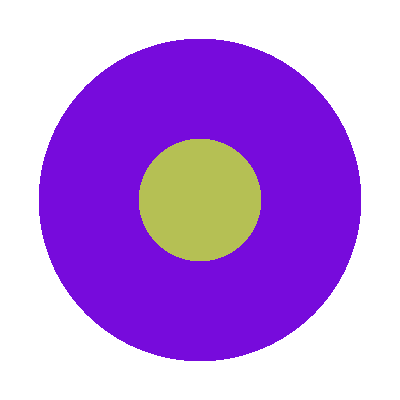
\includegraphics[width=0.3\textwidth]{plot_1}
        \caption{X-Y slice of fuel with reflector.}
        \label{fig:xy}
    \end{figure}

    \begin{figure}[!htb]
        \centering
        
\includegraphics[width=0.3\textwidth ]{plot_2}
        \caption{X-Z slice of fuel with reflector.}
        \label{fig:xz}
    \end{figure}

    The model was run using 200 batches, 10 of which were inactive to allow the Shannon Entropy to converge, with 20,000 particles per batch.
    Additionally, the input file was optimized to search for the critical radius.
    Note that because the radius is directly proportional to the height as given, only one-dimensional optimization is necessary.

    \subsection{Results and Discussion}
    The optimization script returned approximate critical dimensions of 12.25 cm and 22.97 cm for the critical radius and height, respectively.
    These results can be compared to the actual dimensions of the AGN in \cref{tab:mc results}.
    \begin{table}
        \centering
        \begin{tabular}{lll}
            \toprule
            \textbf{Quantity} & \textbf{Simulation Value} & \textbf{Actual Value} \\
            \midrule
            k-effective       & 1.0004 $\pm$ 0.0005       & N/A                   \\
            Radius            & 12.25 cm                  & 12.8 cm               \\
            Height            & 22.97 cm                  & 24 cm                 \\
            \bottomrule
        \end{tabular}
        \caption{OpenMC optimization results.}
        \label{tab:mc results}
    \end{table}

    The Monte Carlo methods proved \emph{much} more accurate than the hand calculations, likely because Monte Carlo methods directly solve the transport equation rather than approximating it.
    The difference of 0.55 cm in critical radii, an error of 4.30\%, can likely be attributed to the simplifications made in the reactor's geometry and composition.
    As can be seen in~\cite{TECHNICALSPECIFICATIONSUNIVERSITY2018}, the reactor core is not a solid cylinder of polyethylene and \ce{UO_2} -- it is multiple shorter cylinders that are stacked together.
    Each cylinder has slight difference material compositions, and these compositions are likely different than the AGN's specifications because some of the fuel has been burned.
    Additionally, the geometry itself is not a perfect cylinder because of the reactor control rods, source, etc., allowing for more absorption and leakage than an ideal system.
    This increases the fuel require to achieve criticality.


    \section{Conclusion}
    The implemented one-group diffusion methods provided unsatisfactory results for both a bare and reflected case, as both models greatly over-predicted the fuel requirements by as much as 82.02\% and as little as 56.17\%.
    Not only is this a waste of space and money, but it is also a grave criticality safety risk for those involved in the construction and operation of the reactor.
    Though hand-calculations have led to successful commercial designs for nuclear reactors, including the AGN itself, the results of this paper showed not only the accuracies they can produce, but also the substantial time investment required.
    Hand calculations can be greatly improved using multigroup methods with diffusion theory, but these methods are cumbersome and prone to errors.

    Given these limitations, Monte Carlo methods offer a more robust alternative with both improved numerical results and workflow.
    The Monte Carlo calculations done by OpenMC proved quite effective at estimating the critical radius and height, even with a simplified geometry, and boasted a relative error of 4.30\%.
    Differences in these results and the actual dimensions of the reactor can be attributed to the age of the fuel (burnup considerations) and imperfect geometry in the model.

    Future work for modeling the AGN would involve improving the OpenMC model to account for the true reactor dimensions and material compositions.


%%%%%%%%%%%%%%%%%%%%%%%%%%%%%%%%%%%%%%%%%%%%%%%%%%%%%%%%%%%%%%%%%%%%%%%%%%%%%%%%
    \bibliographystyle{ans}
    \bibliography{AGN0}
\end{document}

